\section{Case studies}

In this section we present two problems which can naturally be cast in tensor network form.
These problem families are interesting in that they show a transition in complexity when the dimension $d$ carried by the wires of the network is greater than a specific value. The \emph{Jones polynomial} is a prominent \emph{link invariant} in knot theory; here we present the problem of evaluating it at the \emph{lattice roots of unity}.
Subsequently, we briefly look at graph colouring.

\subsection{Jones Polynomial at Lattice Roots of Unity}

% For $d=2,3,4$ it's easy.
% For $d\geq 5$ it's hard.
% Mention Potts and also anyon stuff but the important thing is the tensornet.

A \emph{knot} $K$ is a circle embedded in $\mathbb{R}^3$.
A set of knots tangled together make a \emph{link} $L$.
A link $L$ can be represented by a \emph{link diagram}
by projecting it on to the plane
but retaining the information of \emph{over or under crossings}.
% For example, the trefoil knot linked with an unknot can be drawn as:
% \begin{equation}
% 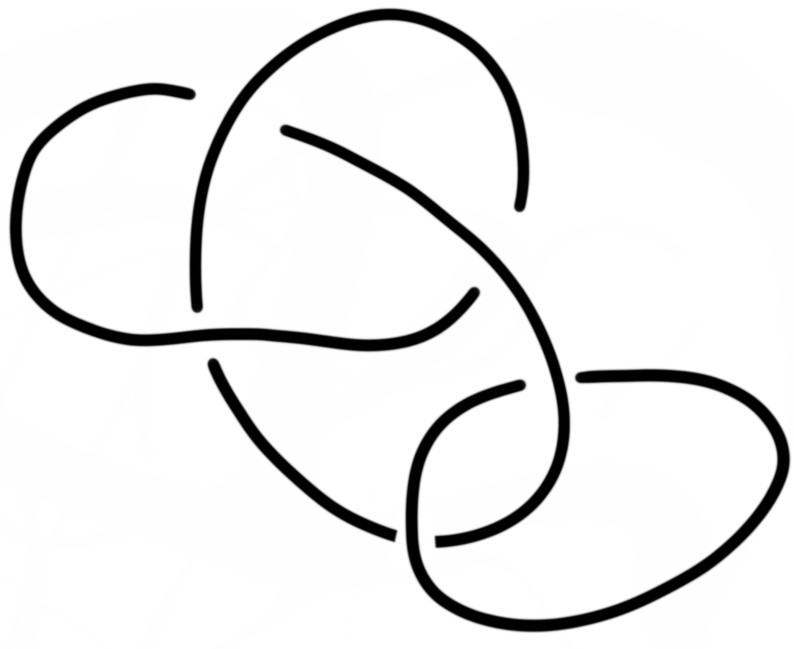
\includegraphics[scale=0.2]{figures/link.jpg}
% \label{eq:link}
% \end{equation}
We say that $L\simeq L'$ iff the diagram of link $L$ can be deformed to that of link $L'$ without cutting or gluing strands, or passing strands through each other.
% there is a sequence of Reidemeister moves from $L$ to $L'$, i.e. reversible local strand deformations that do not change the topology, for example by cutting or gluing strands (see Appendix).
The Jones polynomial $V_L(t)$
is a Laurent polynomial in a variable $t\in\mathbb{C}$
and is a \emph{link invariant}.
This means that
$V_L(t)\neq V_{L'}(t)\Rightarrow L\not\simeq L'$.

In general, computing $V_L(t)$
is exponentially costly in the number of crossings $c$,
something made explicit when one uses the Kauffman bracket method \cite{Kauffman2001}.
Exactly evaluating the Jones polynomial at points $t\in\mathbb{C}$ is \#P-hard,
\emph{except} at the \emph{lattice roots of unity} $\Lambda = \{ \pm 1, \pm i, \pm e^{i 2\pi/3}, \pm e^{i 4\pi/3} \}$,
where it can be evaluated at cost $O(poly(c))$ \cite{jaeger_vertigan_welsh_1990}.


In the context of quantum computation,
additively approximating the Jones polynomial at \emph{non-lattice roots of unity} is the paradigmatic BQP-complete complete problem \cite{Aharonov_2008,kuperberg2014hard}.
Topological quantum computation \cite{Freedman2002,pachos_2012} is the most natural model for such knot theoretic questions. In this model, quantum states are defined in the fusion space of \emph{non-abelian anyons}, emergent quasiparticles with nontrivial exchange statistics arising in two-dimensional exotic phases of matter.
Quantum computation is performed by creating anyons from the vacuum, then braiding them, and finally fusing them back to the vacuum, where braids play the role of unitary gates.
The world-lines of the anyons define a closed braid, i.e. a link.
Such a link encodes a quantum amplitude corresponding to its Jones polynomial evaluated at a lattice root of unity depending on the anyon theory at hand \cite{Witten1989}. 
Specifically, in the case of $\text{SU}(2)_k$ anyons, the Jones polynomial is evaluated at $t(k) = e^{i 2\pi/(2+k)}$ \cite{Rowell_2018}.

Remarkably, the evaluation of the Jones polynomial at certain points can be expressed as an unphysical partition function $Z_{G_L}(d)$ of a $d$-state Potts model with suitable spin-spin interactions \cite{RevModPhys.64.1099}.
This Potts model is defined on a signed graph $G_L$, obtained as follows.
The link diagram is bicoloured checkerboard-style,
then every coloured area is mapped to a vertex and every crossing is mapped to a signed edge according
its orientation relative to the surrounding colours, as in \eqref{eq:link-tn} below.
The Jones polynomial is then equal to this partition function up to an efficiently computable scalar which depends on the link diagram.  
% $V_L(t(d)) \simeq Z_{G_L}(d)$.
The relation between the point $t(d)$ at which the Jones polynomial is evaluated and the dimension $d$ of the spins is $d = t + t^{-1} +2$,
which can be solved for $t(d)$ \cite{PhysRevE.100.033303}.

Note the correspondence between the dimension $d$ in the Potts approach and the level $k$ in the anyon-braiding approach to the Jones polynomial: $\{t(d) | ~ d \in\{1,2,3,4\} \} = \{ t(k) | ~ k\in\{1,2,4,\infty\} \} \subseteq \Lambda$.
This is consistent with the fact that braiding $\text{SU}(2)_2$ anyons (Ising) or $\text{SU}(2)_4$ anyons is not universal (unless the $\text{SU}(2)_4$ anyons are augmented by fusion and measurements \cite{Levaillant_2015}).
% A key observation is that if $d\in\{2,3,4\}$ then $t(d)\in\Lambda$ (the case $d=1$ is trivial \cite{jaeger_vertigan_welsh_1990}).

The partition function $Z_{G_L}(d\in\mathbb{N})$ can be expressed as a closed tensor network in terms of phaseless (green) $d$-dimensional $Z$-spiders connected via wires that go through \emph{$\pm$-boxes} \cite{PhysRevE.100.033303}:
\begin{equation}
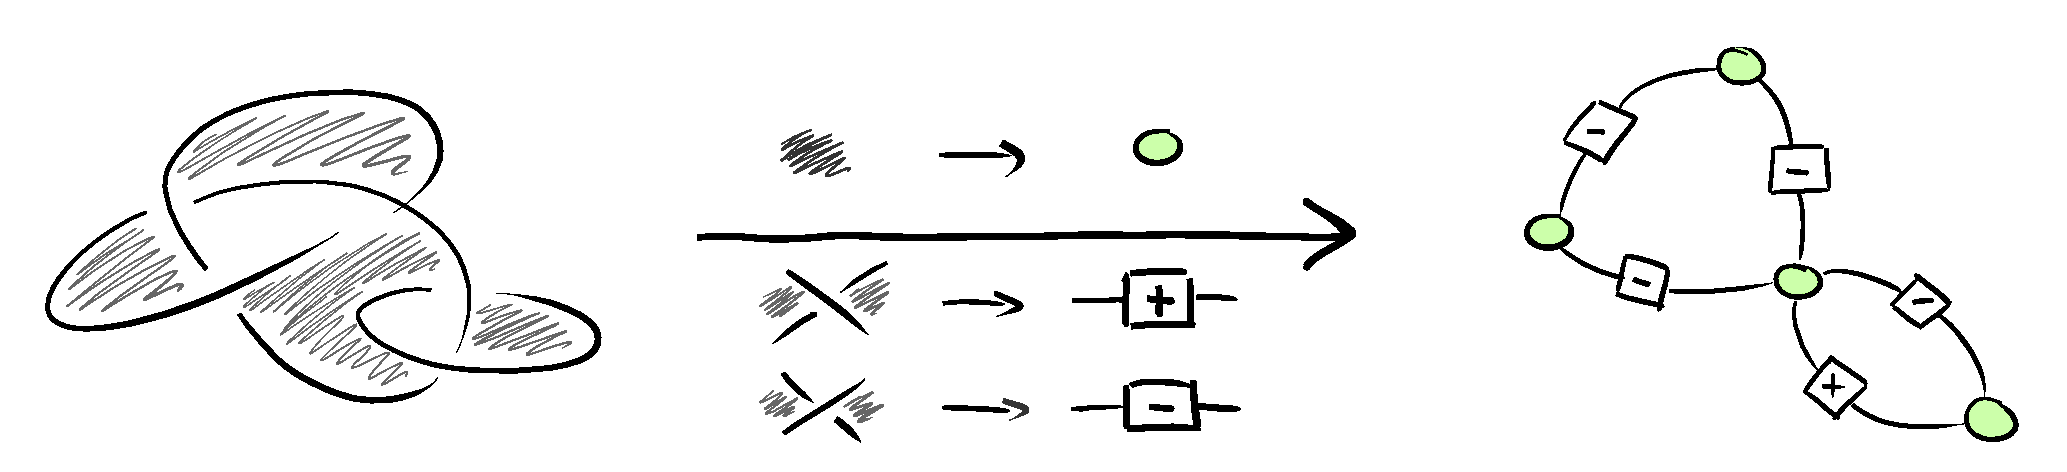
\includegraphics[scale=0.4, valign=c]{figures/link-tn.pdf}
\label{eq:link-tn}
\end{equation}
The $\pm$-boxes have the following concrete interpretation as matrices:
\begin{equation}\label{eq:pm_tensor}
	\left\llbracket \ \tikzfig{pm_maps/pm} \ \right\rrbracket ~~ = ~~  
	\sum_{i,j=0}^{d-1}(1 - (1+t(d)^{\mp 1}) \delta_{ij} ) \ket{i}\bra{j} ~~ = ~~  
	\begin{pmatrix}
		-t(d)^{\mp 1} & 1 & \dots & 1 \\
		1 & -t(d)^{\mp 1} & \dots & 1 \\
		\vdots & \vdots & \ddots & \vdots\\
		1 & 1 & \dots & -t(d)^{\mp 1}
	\end{pmatrix}
\end{equation}
% \begin{remark}\label{rem:qubit_scalar_exactness} 
% 	A small technical remark is in order: the rule set given here is complete for qubit stabilizer quantum mechanics when equality is taken only up to a scalar factor. To achieve completeness under exact equality, a slighly modified rule set would be required, as in (for example) \cite{backens_scalar_exact}. But for our purposes this would be overkill; in order to show that the Jones polynomial of knots at lattice roots of unity is efficiently computable, it suffices to consider the `non-exact' rules - i.e. it suffices to show such a Jones polynomial is efficiently computable up to a scalar factor. But of course to actually compute such a Jones polynomial, we would need to keep track of scalars.
% \end{remark}
% [Move commented out stuff below to appendix proof?]
% DON"T DELETE!!!!!!!!!!!!!!!!!!!!!!!
 % This is because the standard interpretation of diagrams more complex than a single spider can be derived as follows. First a diagram is divided into horizontal strips, then these strips are themselves divided vertically, so that the diagram consists of spiders composed in parallel (side-by-side, written $\otimes$) and in sequence (on top of each other, with legs fused together, written $\circ$). Such a division always exists, though it may require a diagram deformation. For example:
% For spiders $S$ and $T$, we then have:
% \begin{equation}
% 	\left\llbracket S \otimes T \right\rrbracket = \left\llbracket S \right\rrbracket \otimes \left\llbracket T \right\rrbracket 
% \end{equation} 
% \begin{equation}	
% 	\left\llbracket S \circ T \right\rrbracket = \left\llbracket S \right\rrbracket \left\llbracket T \right\rrbracket 
% \end{equation} 
% where on the right hand side of the first equation the $\otimes$ symbol means the Kronecker product of two matrices. Thus a diagram with standard interpretation $T_{2\pm}$ will have one input and one output, while a diagram for $T_{4\pm}$ will have two inputs and two outputs.



We can now express the $\pm$-boxes in the ZX-calculus.
The $\pm$-matrices above for $d \in \{2, 4\}$
are equal up to a scalar to concrete interpretations of \emph{qubit stabilizer} ZX-diagrams, and the $\pm$-matrices for $d=3$ of \emph{qutrit stabilizer} ZX-diagrams (see Appendix \ref{prop:pm_maps_zx_appendix}):
	\begin{equation}
		\left\llbracket \ \tikzfig{pm_maps/pm} \ \right\rrbracket_{d=2} \simeq 
		\left\llbracket \ \tikzfig{pm_maps/q2} \ \right\rrbracket ~, 
		\hspace{30pt}
		\left\llbracket \ \tikzfig{pm_maps/pm} \ \right\rrbracket_{d=3} \simeq
		\left\llbracket \ \tikzfig{pm_maps/q3} \ \right\rrbracket ~,
		\hspace{30pt}
		\left\llbracket \ \tikzfig{pm_maps/pm} \ \right\rrbracket_{d=4} \simeq 
		\left\llbracket \ \tikzfig{pm_maps/q4} \ \right\rrbracket
	\end{equation}
Since these generators decompose as stabilizer diagrams,
$Z_{G_L}(d\in\{2,3,4\})$ can be evaluated \emph{efficiently}
via stabilizer ZX-diagram simplification.
Thus, we recover the known result that evaluating the Jones polynomial at $t\in\Lambda$ is in P.
Computing $Z_{G_L}(d\geq 5)$ is \#P-hard.

%%%%%%%%%%%%%%%%%$ MAYBE SAVE DISCUSSIONS ABOUT WHAT THE SCALAR IS FOR WHEN WE DO THE SCALAR-EXACT VERSION %%%%%%%%%%%%%%%%%%
% Since any ZX-diagram derived from a knot in the manner described in Section \ref{sec:passage} will be closed, this algorithm suffices to prove that the calculation of the Jones polynomial of any knot at the lattice roots of unity $\pm 1$ and $\pm i$ is efficient. This is because reading off the scalar at the end is trivial; either we have the empty diagram, which has standard interpretation $1$, or a single legless $Z$-spider with phase $k\pi$:
% \begin{equation}
% 	\left\llbracket \ \tikzfig{scalars/Z_kpi_1} \ \right\rrbracket = 
% 	\left\llbracket \ \tikzfig{scalars/Z_kpi_2} \ \right\rrbracket = 
% 	( \bra{0} + \bra{1} )( \ket{0} + e^{ik\pi}\ket{1} ) =
% 	1 + e^{ik\pi}
% \end{equation}
% {\bf Furthermore, keeping track of the scalar factors introduced with each application of Theorem \ref{thm:qubit_eliminate_spiders} or Lemma \ref{lem:2_h_edges_vanish} can be done efficiently. [ToDo: proof, if not explicitly doing all this in a scalar-exact fashion. Reference Backens]}

% Having defined the \emph{qutrit} ZX-calculus, we turn our attention back to our tensor network for the Jones polynomial of a knot (ToDo: ref). We are seeking a diagram in the qutrit ZX-calculus that equals (up to a scalar) the matrix $T_{\pm}^{(q)}$ from \eqref{eq:pm_tensor}.

% where we have used $t = \frac{1}{2}(3 - 2 + \sqrt{3(3-4)}) = e^{i\frac{\pi}{3}}$ as in (ToDo: ref). 

% \begin{proposition}\label{prop:pm_map_q3}
% 	Under the standard interpretation as a linear map, the following diagram gives (up to a scalar) the required matrix:
% 	\begin{equation}
% 		\left\llbracket \quad \tikzfig{pm_maps/q3} \quad \right\rrbracket  \simeq
% 		% 2\sqrt{3}e^{\mp i\frac{5\pi}{6}} \ 
% 		\left\llbracket \quad \tikzfig{pm_maps/pm} \quad \right\rrbracket_{q=3} = 
% 		\begin{pmatrix}
% 			e^{\mp i\frac{\pi}{3}} & 1 & 1 \\
% 			1 & e^{\mp i\frac{\pi}{3}} & 1 \\
% 			1 & 1 & e^{\mp i\frac{\pi}{3}} \\
% 		\end{pmatrix}
% 	\end{equation}

% 	\begin{proof}
% 		See Appendix \ref{prop:pm_maps_zx_appendix}.
% 	\end{proof}
% \end{proposition}

% Crucially, the ZX-diagram in Proposition \ref{prop:pm_map_q3} above is a \emph{stabilizer diagram} in the qutrit ZX-calculus - that is, all angles are integer multiples of $\frac{2\pi}{3}$. Therefore if we can find an algorithm analogous to Theorem 5.4 \cite{graph_theoretic_simplification} that efficiently reduces any stabilizer diagram to a trivial one, then we will have shown that the Jones polynomial of any knot at the lattice roots of unity $\pm e^{i\frac{\pi}{3}}$ is efficiently computable. [ToDo: justify the $\pm$]. In the next subsection, we will do exactly that.

% Again - just like in Remark~\ref{rem:qubit_scalar_exactness} - these rules are complete for qutrit stabilizer quantum mechanics when equality is considered only up to a scalar factor; we give the scalar-exact versions (detailed in \citep{qutrit_exact}) so that we can actually compute Jones polynomials later. 




\subsection{Graph Colouring}


Finally, let us briefly look at the \emph{graph colouring problem}. A \emph{$d$-colouring} of a graph $G$ is an assignment of colours $\{1, ..., d\}$ to the vertices of $G$ so that no neighbouring vertices have the same colour. Given a graph $G$ and an integer $d$, we wish to \emph{count} the number of such $d$-colourings. Again, this problem can be interpreted as the zero-temperature
partition function of an antiferromagnetic Potts model (there is an energy cost for adjacent spins to be in the same state).
Through the lens of our graphical exposition we see that counting problems and computing partition functions are essentially the same problem, since both can be straightforwardly encoded as closed tensor networks.

Given a graph $G$, the graph colouring problem can be encoded as a ZX-diagram as follows. Every vertex of the graph is mapped to a $d$-dimensional phaseless (green) $Z$-spider.
Every edge is mapped to a wire connecting the spiders
which goes through an $X$-box.
\begin{equation}\label{eq:G-tn}
	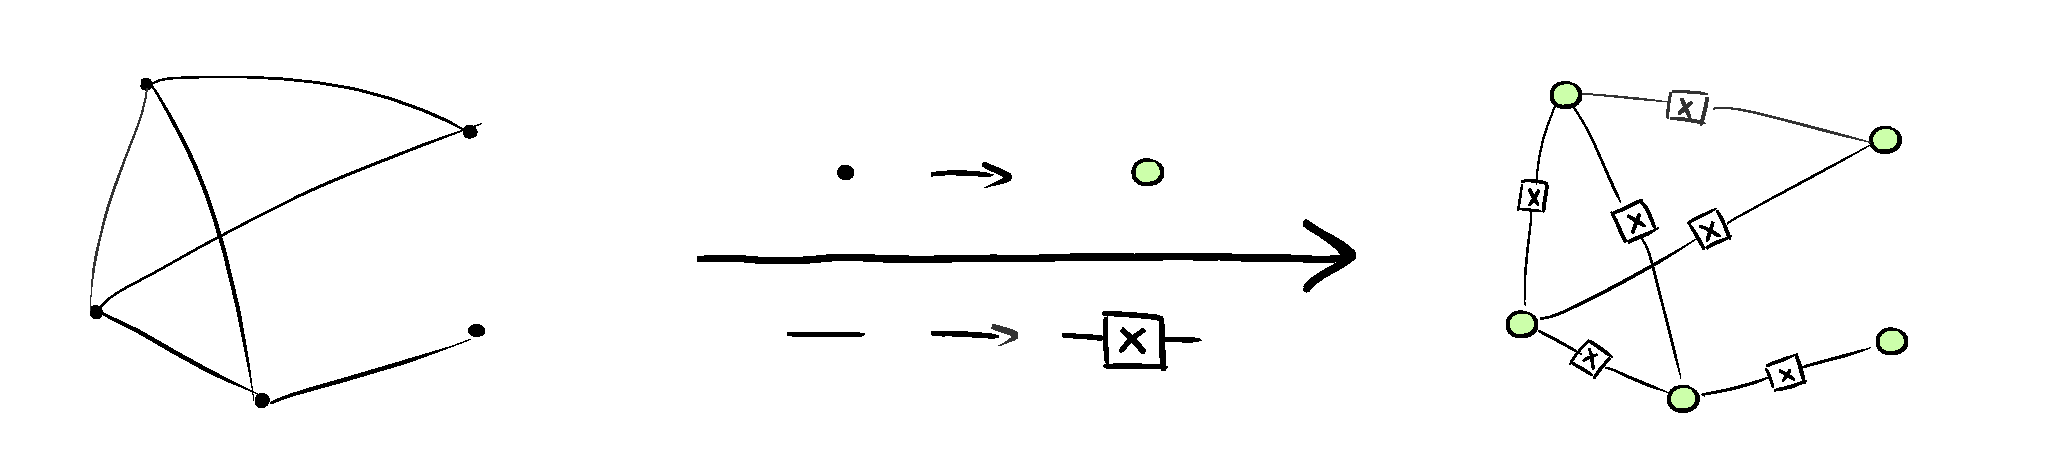
\includegraphics[scale=0.4, valign=c]{figures/G-tn.pdf}
\end{equation}
The $X$-boxes have the following concrete interpretation (as special case of the $\pm$-boxes, where $t=0$):
\begin{equation}\label{eq:X_tensor}
	\left\llbracket \ \tikzfig{pm_maps/x} \ \right\rrbracket ~~ = ~~  
	\sum_{i,j=0}^{d-1} (1 -  \delta_{ij} ) \ket{i}\bra{j} ~~ = ~~  
	\begin{pmatrix}
		0 & 1 & \dots & 1 \\
		1 & 0 & \dots & 1 \\
		\vdots & \vdots & \ddots & \vdots\\
		1 & 1 & \dots & 0
	\end{pmatrix}
\end{equation}

Counting k-colourings for $k\geq 3$ is a canonical \#P-complete problem,
while for $k=0,1,2$ the problem is in P \cite{jaeger_vertigan_welsh_1990}.
And indeed, for $d=2$ the $X$-matrix is just the Pauli X, and so the problem reduces to simplifying a stabilizer diagram,
which can be done efficiently.
However, for $d=3$ the $X$-matrix cannot be expressed as a stabilizer qutrit diagram.
	\begin{equation}\label{eq:XmatricesinZX}
		\left\llbracket \ \tikzfig{pm_maps/x} \ \right\rrbracket_{d=2} \simeq \left\llbracket \ \tikzfig{pm_maps/q2x} \ \right\rrbracket  \quad, 
		\qquad\quad
		\left\llbracket \quad \tikzfig{pm_maps/x} \quad \right\rrbracket_{d=3} \not\simeq
		\left\llbracket \quad \tikzfig{pm_maps/q3x} \quad \right\rrbracket~~,~~~~\forall a,b\in\{0,1,2\}
	\end{equation}
Thus it is not expected that there exists an efficient simplification strategy for the corresponding qutrit ZX-diagram. This is consistent with the fact that counting 3-colourings is \#P-complete.
